% questions.tex —— 1994 年·上海卷 · 题目内容片段（无答案）
% 由 tools/generate_projects.py 依来源总账自 1994/1994_数学真题_上海_试题.md 生成，勿手改（改源 MD 后重跑）


考生注意：这份试卷共有 26 道试题，满分 150 分。

\gkpart{一、填空题}

本大题满分 30 分，共有 10 题，只要求直接填写结果。每个空格填对得 3 分，否则一律得零分。

\begin{question}
\gkti{1}不等式 $|x+1|<1$ 的解是\gkblank{}。

\end{question}
\begin{question}
\gkti{2}计算：$\sin\left(\dfrac12\arccos\dfrac18\right)=$\gkblank{}。

\end{question}
\begin{question}
\gkti{3}以点 $C(-2,3)$ 为圆心且与 $y$ 轴相切的圆的方程是\gkblank{}。

\end{question}
\begin{question}
\gkti{4}方程 $\log_3(x-1)=\log_9(x+5)$ 的解是\gkblank{}。

\end{question}
\begin{question}
\gkti{5}有一个实心圆锥体的零部件，它的轴截面是边长为 $10$ 厘米的等边三角形。现要在它的整个表面镀上一层防腐材料，已知每平方厘米的工料价为 $0.10$ 元，则需要费用\gkblank{}元（$\pi$ 取 $3.2$）。

\end{question}
\begin{question}
\gkti{6}函数 $y=\sqrt{x^2-1}\ (x\le -1)$ 的反函数是\gkblank{}。

\end{question}
\begin{question}
\gkti{7}双曲线 $\dfrac{y^2}{2}-x^2=1$ 的两个焦点的坐标是\gkblank{}。

\end{question}
\begin{question}
\gkti{8}$\left(x^3-\dfrac2{x^2}\right)^5$ 的展开式中 $x^5$ 的系数是\gkblank{}（结果用数值表示）。

\end{question}
\begin{question}
\gkti{9}函数 $y=\sin 2x-2\cos^2x$ 的最大值是\gkblank{}。

\end{question}
\begin{question}
\gkti{10}函数

\nopagebreak[4]
\[
y=\frac{\sin 2x+\sin\left(2x+\frac\pi3\right)}{\cos 2x+\cos\left(2x+\frac\pi3\right)}
\]

的最小正周期是\gkblank{}。

\end{question}
\gkpart{二、选择题}

本大题满分 30 分，共有 10 题。每题都给出代号为 A、B、C、D 的四个结论，其中有且只有一个结论是正确的，必须把正确结论的代号写在题后的圆括号内。选对得 3 分，不选、选错或者选出的代号超过一个（不论是否写在圆括号内），一律得零分。

\Needspace{0.4\textheight}
\begin{question}
\gkti{11}当 $a>1$ 时，函数 $y=\log_a x$ 和 $y=(1-a)x$ 的图象只可能是（　）。
\nopagebreak[4]
\begin{center}% 依固定扫描件第 1 页四种函数图象选项转绘；形态示意，不宣称精确比例。
\begin{center}
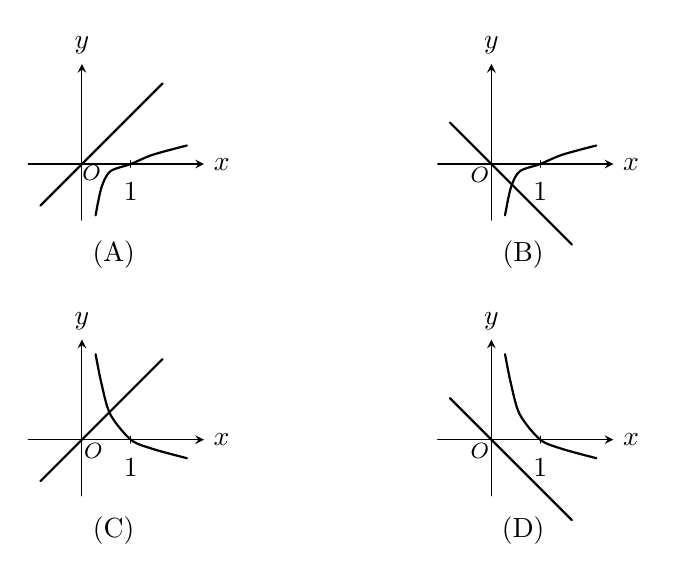
\begin{tikzpicture}[x=0.62cm,y=0.62cm,>=stealth,line cap=round,line join=round]
\foreach \xshift/\yshift/\label/\lineup/\logup/\originplace/\originsep in {
  0/3.5/A/1/1/right/0, 5.2/3.5/B/-1/1/left/0.6,
  0/0/C/1/-1/right/0.6, 5.2/0/D/-1/-1/left/0.6} {
  \begin{scope}[xshift=\xshift cm,yshift=\yshift cm]
    \draw[->] (-1.1,0)--(2.5,0) node[right] {$x$};
    \draw[->] (0,-1.15)--(0,2.05) node[above] {$y$};
    \draw (1,0.07)--(1,-0.07) node[below=2pt] {$1$};
    \node[below \originplace,font=\footnotesize,inner sep=\originsep pt,yshift=-0.4pt] at (0,0) {$O$};
    \ifnum\lineup=1
      \draw[thick] (-0.85,-0.85)--(1.65,1.65);
    \else
      \draw[thick] (-0.85,0.85)--(1.65,-1.65);
    \fi
    \ifnum\logup=1
      \draw[thick] plot[smooth] coordinates {(0.28,-1.05) (0.4,-0.48) (0.58,-0.15) (1,0) (1.45,0.19) (2.15,0.38)};
    \else
      \draw[thick] plot[smooth] coordinates {(0.28,1.75) (0.4,1.15) (0.58,0.52) (1,0) (1.45,-0.19) (2.15,-0.38)};
    \fi
    \node[below] at (0.65,-1.38) {(\label)};
  \end{scope}
}
\end{tikzpicture}
\end{center}
\end{center}
\nopagebreak[4]
\end{question}
\begin{question}
\gkti{12}如果 $0<a<1$，那么下列不等式中正确的是（　）。

\begin{gkopts}(2)
\task A．$(1-a)^{1/3}>(1-a)^{1/2}$；
\task B．$\log_{1-a}(1+a)>0$；
\task C．$(1-a)^3>(1+a)^2$；
\task D．$(1-a)^{1+a}>1$。
\end{gkopts}

\end{question}
\begin{question}
\gkti{13}已知点 $P$ 的极坐标为 $(1,\pi)$，那么过点 $P$ 且垂直于极轴的直线的极坐标方程为（　）。

\begin{gkopts}(1)
\task A．$\rho=1$；B．$\rho=\cos\theta$；C．$\rho=-\dfrac1{\cos\theta}$；D．$\rho=\dfrac1{\cos\theta}$。
\end{gkopts}

\end{question}
\begin{question}
\gkti{14}已知 $a,b$ 是异面直线，直线 $c$ 平行于直线 $a$，那么 $c$ 与 $b$（　）。

\begin{gkopts}(1)
\task A．一定是异面直线；B．一定是相交直线；C．不可能是平行直线；D．不可能是相交直线。
\end{gkopts}

\end{question}
\begin{question}
\gkti{15}设 $I$ 是全集，集合 $P,Q$ 满足 $P\subset Q$，那么下面的结论中错误的是（　）。

\begin{gkopts}(1)
\task A．$P\cup Q=Q$；B．$\overline P\cup Q=I$；C．$P\cap\overline Q=\varnothing$；D．$\overline P\cap\overline Q=\overline P$。
\end{gkopts}

\end{question}
\begin{question}
\gkti{16}设复数 $z=-\dfrac12+\dfrac{\sqrt3}{2}i$（$i$ 为虚数单位），则满足等式 $z^n=z$，且大于 $1$ 的正整数 $n$ 中最小的是（　）。

\begin{gkopts}(2)
\task A．$3$；B．$4$；C．$6$；D．$7$。
\end{gkopts}

\end{question}
\begin{question}
\gkti{17}设 $a,b$ 是平面 $\alpha$ 外的任意两条线段，那么“$a,b$ 的长相等”是“$a,b$ 在平面 $\alpha$ 内的射影长相等”的（　）。

\begin{gkopts}(1)
\task A．非充分条件也非必要条件；B．充分必要条件；C．必要条件而非充分条件；D．充分条件而非必要条件。
\end{gkopts}

\end{question}
\begin{question}
\gkti{18}计划在某画廊展出 $10$ 幅不同的画，其中 $1$ 幅水彩画、$4$ 幅油画、$5$ 幅国画，排成一行陈列。要求同一品种的画必须连在一起，并且水彩画不放在两端，那么不同陈列方式有（　）。

\begin{gkopts}(1)
\task A．$P_4^4\cdot P_5^5$ 种；B．$P_3^3\cdot P_4^4\cdot P_5^5$ 种；C．$C_3^1\cdot P_4^4\cdot P_5^5$ 种；D．$P_2^2\cdot P_4^4\cdot P_5^5$ 种。
\end{gkopts}

\end{question}
\begin{question}
\gkti{19}在直角坐标系 $xOy$ 中，曲线 $C$ 的方程是 $y=\cos x$。现平移坐标系，把原点移到点 $O'\left(\dfrac\pi2,-\dfrac\pi2\right)$，那么在坐标系 $x'O'y'$ 中，曲线 $C$ 的方程是（　）。

\begin{gkopts}(1)
\task A．$y'=\sin x'+\dfrac\pi2$；B．$y'=-\sin x'+\dfrac\pi2$；C．$y'=\sin x'-\dfrac\pi2$；D．$y'=-\sin x'-\dfrac\pi2$。
\end{gkopts}

\end{question}
\begin{question}
\gkti{20}某个命题与自然数 $n$ 有关。如果当 $n=k\ (k\in\mathbb N)$ 时该命题成立，那么可推得当 $n=k+1$ 时该命题也成立。现已知当 $n=5$ 时该命题不成立，那么可推得（　）。

\begin{gkopts}(1)
\task A．当 $n=6$ 时该命题不成立；B．当 $n=6$ 时该命题成立；C．当 $n=4$ 时该命题不成立；D．当 $n=4$ 时该命题成立。
\end{gkopts}

\end{question}
\gkpart{三、解答题}

本大题满分 36 分，共有 3 题，解答下列各题必须写出必要的步骤。

\begin{question}
\gkti{21}（本题满分 $12$ 分）已知 $\sin\alpha=\dfrac35$，$\alpha\in\left(\dfrac\pi2,\pi\right)$，$\operatorname{tg}(\pi-\beta)=\dfrac12$，求 $\operatorname{tg}(\alpha-2\beta)$ 的值。

\end{question}
\begin{question}
\gkti{22}（本题满分 $12$ 分）设 $w$ 为复数，它的辐角的主值为 $\dfrac{3\pi}4$，且 $\dfrac{(\overline w)^2-4}{w}$ 为实数，求复数 $w$。

\Needspace{0.4\textheight}
\end{question}
\begin{question}
\gkti{23}（本题满分 $12$ 分）本题共有 $2$ 个小题，第 $1$ 小题满分 $6$ 分，第 $2$ 小题满分 $6$ 分。

如图，在梯形 $ABCD$ 中，$AD\parallel BC$，$\angle ABC=\dfrac\pi2$，$AB=a$，$AD=3a$，且 $\angle ADC=\arcsin\dfrac{\sqrt5}{5}$。又 $PA\perp$ 平面 $ABCD$，$PA=a$。求：
\nopagebreak[4]
\begin{center}% 依固定扫描件第 2 页转绘梯形与棱锥的拓扑关系；不表示精确比例。
\begin{center}
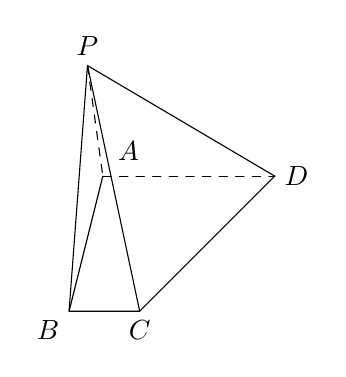
\begin{tikzpicture}[x=0.78cm,y=0.78cm,>=stealth,line cap=round,line join=round]
  \coordinate (B) at (0,0);
  \coordinate (A) at (0.55,2.2);
  \coordinate (C) at (1.15,0);
  \coordinate (D) at (3.35,2.2);
  \coordinate (P) at (0.3,4.0);
  \draw (A)--(B)--(C)--(D);
  \draw[dashed] (A)--(D);
  \draw (P)--(B) (P)--(C) (P)--(D);
  \draw[dashed] (P)--(A);
  \node[above right,xshift=2pt,yshift=2pt] at (A) {$A$};
  \node[below left] at (B) {$B$};
  \node[below] at (C) {$C$};
  \node[right] at (D) {$D$};
  \node[above] at (P) {$P$};
\end{tikzpicture}
\end{center}
\end{center}
\nopagebreak[4]
（1） 二面角 $P-CD-A$ 的大小（用反三角函数表示）；

（2） 点 $A$ 到平面 $PBC$ 的距离。

\end{question}
\gkpart{四、解答题}

本大题满分 54 分，共有 3 题，解答下列各题必须写出必要的步骤。

\begin{question}
\gkti{24}（本题满分 $16$ 分）本题共有 $2$ 个小题，第 $1$ 小题满分 $6$ 分，第 $2$ 小题满分 $10$ 分。

设椭圆的中心为原点 $O$，一个焦点为 $F(0,1)$，长轴和短轴的长度之比为 $t$。

（1） 求椭圆的方程；

\Needspace{5\baselineskip}
（2） 设经过原点且斜率为 $t$ 的直线与椭圆在 $y$ 轴右边部分的交点为 $Q$，点 $P$ 在该直线上，且
\nopagebreak[4]
\[
\frac{|OP|}{|OQ|}=t\sqrt{t^2-1}\mbox{。}
\]
当 $t$ 变化时，求点 $P$ 的轨迹方程，并说明轨迹是什么图形。

\end{question}
\begin{question}
\gkti{25}（本题满分 $18$ 分）本题共有 $2$ 个小题，第 $1$ 小题满分 $10$ 分，第 $2$ 小题满分 $8$ 分。

在直角坐标系中，设矩形 $OPQR$ 的顶点按逆时针顺序依次为 $O(0,0)$、$P(1,t)$、$Q(1-2t,2+t)$、$R(-2t,2)$，其中 $t\in(0,+\infty)$。

（1） 求矩形 $OPQR$ 在第一象限部分的面积 $S(t)$；

（2） 确定函数 $S(t)$ 的单调区间，并加以证明。

\end{question}
\begin{question}
\gkti{26}（本题满分 $20$ 分）本题共有 $3$ 个小题，第 $1$ 小题满分 $4$ 分，第 $2$ 小题满分 $8$ 分，第 $3$ 小题满分 $8$ 分。

已知数列 $\{a_n\}$ 满足条件：$a_1=1$，$a_2=r\ (r>0)$，且 $\{a_na_{n+1}\}$ 是公比为 $q\ (q>0)$ 的等比数列。设 $b_n=a_{2n-1}+a_{2n}\ (n=1,2,\ldots)$。

\Needspace{5\baselineskip}
（1） 求出使不等式
\nopagebreak[4]
\[
a_na_{n+1}+a_{n+1}a_{n+2}>a_{n+2}a_{n+3}\quad(n\in\mathbb N)
\]
成立的 $q$ 的取值范围；

（2） 求 $b_n$ 和 $\displaystyle\lim_{n\to\infty}\dfrac1{S_n}$，其中 $S_n=b_1+b_2+\cdots+b_n$；

\Needspace{5\baselineskip}
（3） 设 $r=2^{19.2}-1$，$q=\dfrac12$，求数列
\nopagebreak[4]
\[
\left\{\frac{\log_2 b_{n+1}}{\log_2 b_n}\right\}
\]
的最大项和最小项的值。

\end{question}